\documentclass{article}
\usepackage{graphicx}
\graphicspath{{partials/}{graphics}!virker ikke endnu
\begin{document}
\section{designovervejelser}
Vi har valget at lave et program der planlægger skema for udskolingssektoren på en givende skole. Vi har valgt det skal være udskoling, altså 7, 8 og 9 klasse, for at kunne simulerede at lærerne kan have klasser på tværs af klassetrinene, og der ved vise at software løsningen kan løse problemet med sammenhængene forberedelsestimer for lærerne. Derudover skal programmet kunne planlægge skemaerne således at det er muligt at have samarbejde på tværs af parallel klasserne.  Da det er udskoling der arbejdes videre med, skal der specificeres hvilke parametre der gælder for disse klassetrin. Alle klassetrinene skal undervises i dansk, idræt, matematik, engelsk, historie, biologi, geografi, fysik og kemi, tysk eller fransk, derudover skal de have mulighed for at have et valgfag, det kunne f.eks. være fransk, billedkunst eller musik, alt efter hvad skolen har mulighed for at tilbyde. På syvende klassetrin er der også et praktisk fag som håndarbejde, sløjd eller hjemmekundskab på skemaet. De har til gengæld ikke kristendom på skemaet, da de har konfirmationsforberedelse. ikke Det fulde time antal for de forskellige fag kan ses på nedenstående skema(indsæt billedet: antal af timer på et år.png):
\begin{figure}[h!]
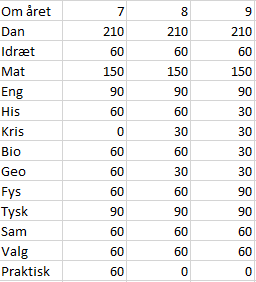
\includegraphics[width=\linewidth]{antalaftimerpaaetaar.png}
\caption{Skema over antallet af timer 7, 8 og 9 har på et helt år}
\label{Fig: XXX}
\end{figure}

Ugeligt vil det passe med følgende(indsæt billedet: antal timer på en uge.png):
\begin{figure}[h!]
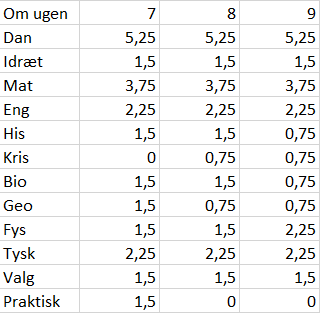
\includegraphics[width=\linewidth]{antalaftimerpaaenuge.png}
\caption{Skema over antallet af timer 7, 8 og 9 har på en uge}
\label{Fig: XXX2}
\end{figure}

Derudover skal programmet opfylde de specifikke krav der bliver stillet af Sofiendahlskolen. Disse krav er at alle de tunge fag, som 
\end{document}